\documentclass{beamer}\usepackage[]{graphicx}\usepackage[]{color}
%% maxwidth is the original width if it is less than linewidth
%% otherwise use linewidth (to make sure the graphics do not exceed the margin)
\makeatletter
\def\maxwidth{ %
  \ifdim\Gin@nat@width>\linewidth
    \linewidth
  \else
    \Gin@nat@width
  \fi
}
\makeatother

\definecolor{fgcolor}{rgb}{1, 0.894, 0.769}
\newcommand{\hlnum}[1]{\textcolor[rgb]{0.824,0.412,0.118}{#1}}%
\newcommand{\hlstr}[1]{\textcolor[rgb]{1,0.894,0.71}{#1}}%
\newcommand{\hlcom}[1]{\textcolor[rgb]{0.824,0.706,0.549}{#1}}%
\newcommand{\hlopt}[1]{\textcolor[rgb]{1,0.894,0.769}{#1}}%
\newcommand{\hlstd}[1]{\textcolor[rgb]{1,0.894,0.769}{#1}}%
\newcommand{\hlkwa}[1]{\textcolor[rgb]{0.941,0.902,0.549}{#1}}%
\newcommand{\hlkwb}[1]{\textcolor[rgb]{0.804,0.776,0.451}{#1}}%
\newcommand{\hlkwc}[1]{\textcolor[rgb]{0.78,0.941,0.545}{#1}}%
\newcommand{\hlkwd}[1]{\textcolor[rgb]{1,0.78,0.769}{#1}}%
\let\hlipl\hlkwb

\usepackage{framed}
\makeatletter
\newenvironment{kframe}{%
 \def\at@end@of@kframe{}%
 \ifinner\ifhmode%
  \def\at@end@of@kframe{\end{minipage}}%
  \begin{minipage}{\columnwidth}%
 \fi\fi%
 \def\FrameCommand##1{\hskip\@totalleftmargin \hskip-\fboxsep
 \colorbox{shadecolor}{##1}\hskip-\fboxsep
     % There is no \\@totalrightmargin, so:
     \hskip-\linewidth \hskip-\@totalleftmargin \hskip\columnwidth}%
 \MakeFramed {\advance\hsize-\width
   \@totalleftmargin\z@ \linewidth\hsize
   \@setminipage}}%
 {\par\unskip\endMakeFramed%
 \at@end@of@kframe}
\makeatother

\definecolor{shadecolor}{rgb}{.97, .97, .97}
\definecolor{messagecolor}{rgb}{0, 0, 0}
\definecolor{warningcolor}{rgb}{1, 0, 1}
\definecolor{errorcolor}{rgb}{1, 0, 0}
\newenvironment{knitrout}{}{} % an empty environment to be redefined in TeX

\usepackage{alltt}
\usepackage{../371g-slides}
\usepackage{}
\title{Time Series: Autocorrelation}
\subtitle{Lecture 25}
\author{STA 371G}
\IfFileExists{upquote.sty}{\usepackage{upquote}}{}
\begin{document}
  
  

  \frame{\maketitle}

  % Show outline at beginning of each section
  \AtBeginSection[]{
    \begin{frame}<beamer>
      \tableofcontents[currentsection]
    \end{frame}
  }

  %%%%%%% Slides start here %%%%%%%

  \begin{darkframes}

    \begin{frame}{Predicting oil prices}
      \fontsize{10}{10}\selectfont
      \begin{center}
        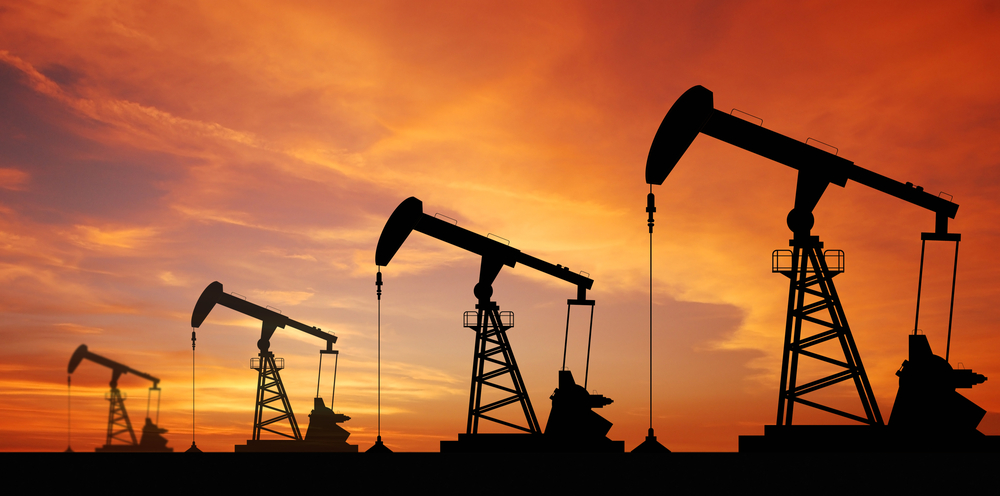
\includegraphics[width=2.8in]{pumpjack} \\
      \end{center}

      \vspace{-0.1in}
      \begin{columns}[onlytextwidth]
        \column{.4\textwidth}
            \begin{center}
              \begin{tabular}{ll}
              \hline
              Date & Oil price (\$) \\
              \hline
              1/1/2013 & 112.98  \\
              1/1/2014 & 107.94 \\
              1/1/2015 & 55.38 \\
              1/1/2016 & 36.85 \\
              1/1/2017 & 55.05 \\
              1/1/2018 & ? \\
              \hline
            \end{tabular}
          \end{center} \pause

        \column{.6\textwidth}
          \begin{itemize}[<+->]
            \item What's the best prediction of the price of oil on January 1?
            \item Does next year's price depend on this year's?
          \end{itemize}
      \end{columns}
      \lc
    \end{frame}




    \begin{frame}{Time series}
      In a \alert{time series,} data are not necessarily independent. (Often it is not!) \pause
      \bigskip

      Time series:
      \begin{itemize}
        \item A sequence of measurements of the same variable collected over time.
        \item The measurements are made at regular time intervals (most commonly daily, weekly, monthly, quarterly, or yearly).
        \item The variances are not necessarily constant over time either.
      \end{itemize}
    \end{frame}



    \begin{frame}{Some examples}
      \begin{itemize}
        \item S\&P 500 index (or any stock price)
        \item iPhone sales worldwide
        \item U.S. unemployment rate
        \item U.S. inflation rate
        \item Crime rate in Austin
      \end{itemize} \pause
      \bigskip
      Any of these could be measured at weekly, monthly, yearly etc. intervals; and each would be a different time series.
    \end{frame}


\begin{frame}[fragile]{Oil Prices 1979-2004}
      \fontsize{8}{8}\selectfont
\begin{knitrout}
\definecolor{shadecolor}{rgb}{0.137, 0.137, 0.137}\begin{kframe}
\begin{alltt}
\hlcom{# Convert the data into a time series object}
\hlstd{price} \hlkwb{<-} \hlkwd{ts}\hlstd{(oil}\hlopt{$}\hlstd{price,} \hlkwc{start}\hlstd{=}\hlnum{1979}\hlstd{,} \hlkwc{frequency}\hlstd{=}\hlnum{1}\hlstd{)}
\hlcom{# Frequency: # of data points per year}
\hlkwd{plot}\hlstd{(price)}
\end{alltt}
\end{kframe}
\input{/tmp/figures/unnamed-chunk-2-1.tikz}

\end{knitrout}
\end{frame}



\begin{frame}[fragile]{Oil Prices 1979-2004}
      We argued that oil prices are not independent year-over-year. \pause To predict the oil price in a given year, can we use the previous year's price? \pause

      \begin{center}
        $y_t$: The oil price at the end of the year $t$ \pause\bigskip

        \begin{tabular}{lll}
          \hline
            $t$ & $y_t$ &  $y_{t-1}$\\
          \hline
          \ldots & \ldots & \ldots \\
          1999	& 16.56 & 11.91 \\
          2000 &	27.39 & 16.56  \\
          2001	& 23 & 27.39 \\
          2002	& 22.81 & 23 \\
          \ldots & \ldots & \ldots \\
          \hline
        \end{tabular}
      \end{center}
      \pause

      $y_{t-1}$ column is obtained by shifting $y_t$ by 1. \pause

      The \alert{lag} between $y_t$ and $y_{t-1}$ is one time-step.

\end{frame}


\begin{frame}[fragile]{Compute one-lag time series}
      \fontsize{10}{10}\selectfont
\begin{knitrout}
\definecolor{shadecolor}{rgb}{0.137, 0.137, 0.137}\begin{kframe}
\begin{alltt}
\hlcom{# Create lag 1 time series.}
\hlstd{priceL1} \hlkwb{<-} \hlkwd{lag}\hlstd{(price,} \hlkwc{k}\hlstd{=}\hlopt{-}\hlnum{1}\hlstd{)}
\hlcom{# Put them together}
\hlstd{price_all} \hlkwb{<-} \hlkwd{cbind}\hlstd{(}\hlkwc{price}\hlstd{=price,} \hlkwc{priceL1}\hlstd{=priceL1)}
\hlstd{price_all[}\hlnum{1}\hlopt{:}\hlnum{5}\hlstd{,]}
\end{alltt}
\begin{verbatim}
     price priceL1
[1,] 25.10      NA
[2,] 37.42   25.10
[3,] 35.75   37.42
[4,] 31.83   35.75
[5,] 29.08   31.83
\end{verbatim}
\end{kframe}
\end{knitrout}
      \pause

      \texttt{priceL1} in the first row is \texttt{NA} because we did not have data from 1978 to put under $y_{t-1}$ column of 1979.
\end{frame}




    \begin{frame}{Linear regression model}
      The simple linear regression model is:
        \[
          y_t = \beta_0 + \beta_1 y_{t-1} + \epsilon_t
        \]
      \pause
      Note that we obtained our predictor from the response itself, lagged 1 time step!
    \end{frame}

\begin{frame}[fragile]%{Linear regression model}
      \fontsize{9}{9}\selectfont
      When we use such a model, we expect to see a linear relation between the predictor and the response. Let's see if there is such a relation! \pause
\begin{knitrout}
\definecolor{shadecolor}{rgb}{0.137, 0.137, 0.137}\begin{kframe}
\begin{alltt}
\hlkwd{plot}\hlstd{(price} \hlopt{~} \hlstd{priceL1,} \hlkwc{xy.labels}\hlstd{=F,} \hlkwc{xy.lines}\hlstd{=F)}
\end{alltt}
\end{kframe}
\input{/tmp/figures/unnamed-chunk-4-1.tikz}

\end{knitrout}
      \pause
      The oil prices seem to be correlated with its first lag! \pause This is called \alert{autocorrelation.}

\end{frame}


\begin{frame}[fragile]%{Linear regression model}
      \fontsize{9}{9}\selectfont
\begin{knitrout}
\definecolor{shadecolor}{rgb}{0.137, 0.137, 0.137}\begin{kframe}
\begin{alltt}
\hlstd{model} \hlkwb{<-} \hlkwd{lm}\hlstd{(price} \hlopt{~} \hlstd{priceL1,} \hlkwc{data}\hlstd{=price_all)}
\hlkwd{summary}\hlstd{(model)}
\end{alltt}
\begin{verbatim}

Call:
lm(formula = price ~ priceL1, data = price_all)

Residuals:
     Min       1Q   Median       3Q      Max 
-11.9046  -2.9505  -0.8162   1.6303  12.4595 

Coefficients:
            Estimate Std. Error t value Pr(>|t|)    
(Intercept)   5.8724     3.8389   1.530 0.139722    
priceL1       0.7605     0.1642   4.632 0.000116 ***
---
Signif. codes:  0 '***' 0.001 '**' 0.01 '*' 0.05 '.' 0.1 ' ' 1

Residual standard error: 5.454 on 23 degrees of freedom
  (2 observations deleted due to missingness)
Multiple R-squared:  0.4827,	Adjusted R-squared:  0.4602 
F-statistic: 21.46 on 1 and 23 DF,  p-value: 0.0001164
\end{verbatim}
\end{kframe}
\end{knitrout}
      \pause
      This is a first-order autoregressive, \alert{AR(1)}, model.
      \note{LC questions 2 and 3}
\end{frame}


\begin{frame}[fragile]{AR(2) model}
      \fontsize{8}{8}\selectfont
      Let's try to add one more lag.
\begin{knitrout}
\definecolor{shadecolor}{rgb}{0.137, 0.137, 0.137}\begin{kframe}
\begin{alltt}
\hlcom{# Create lag 2 time series.}
\hlstd{priceL2} \hlkwb{<-} \hlkwd{lag}\hlstd{(price,} \hlkwc{k}\hlstd{=}\hlopt{-}\hlnum{2}\hlstd{)}
\hlcom{# Put them together}
\hlstd{price_all} \hlkwb{<-} \hlkwd{cbind}\hlstd{(}\hlkwc{price}\hlstd{=price,} \hlkwc{priceL1}\hlstd{=priceL1,} \hlkwc{priceL2}\hlstd{=priceL2)}
\hlstd{price_all[}\hlnum{1}\hlopt{:}\hlnum{5}\hlstd{,]}
\end{alltt}
\begin{verbatim}
     price priceL1 priceL2
[1,] 25.10      NA      NA
[2,] 37.42   25.10      NA
[3,] 35.75   37.42   25.10
[4,] 31.83   35.75   37.42
[5,] 29.08   31.83   35.75
\end{verbatim}
\end{kframe}
\end{knitrout}
      \pause
      The model then becomes:
      $$
        y_t = \beta_0 + \beta_1 y_{t-1} + \beta_2 y_{t-2} + \epsilon_t
      $$
\end{frame}



\begin{frame}[fragile]{AR(2) model}
      \fontsize{8}{8}\selectfont
\begin{knitrout}
\definecolor{shadecolor}{rgb}{0.137, 0.137, 0.137}\begin{kframe}
\begin{alltt}
  \hlstd{model} \hlkwb{<-} \hlkwd{lm}\hlstd{(price} \hlopt{~} \hlstd{priceL1} \hlopt{+} \hlstd{priceL2,} \hlkwc{data}\hlstd{=price_all)}
  \hlkwd{summary}\hlstd{(model)}
\end{alltt}
\begin{verbatim}

Call:
lm(formula = price ~ priceL1 + priceL2, data = price_all)

Residuals:
     Min       1Q   Median       3Q      Max 
-10.6861  -3.0937   0.7269   2.3375  10.9071 

Coefficients:
            Estimate Std. Error t value Pr(>|t|)    
(Intercept)   7.1749     3.7363   1.920 0.068505 .  
priceL1       0.8427     0.2073   4.064 0.000557 ***
priceL2      -0.1646     0.2094  -0.786 0.440530    
---
Signif. codes:  0 '***' 0.001 '**' 0.01 '*' 0.05 '.' 0.1 ' ' 1

Residual standard error: 4.911 on 21 degrees of freedom
  (4 observations deleted due to missingness)
Multiple R-squared:  0.5411,	Adjusted R-squared:  0.4974 
F-statistic: 12.38 on 2 and 21 DF,  p-value: 0.0002807
\end{verbatim}
\end{kframe}
\end{knitrout}
\end{frame}



\begin{frame}[fragile]{AR(2) model}
      \begin{itemize}
      \item \texttt{priceL2} is not statistically significant, if we include \texttt{priceL1}.
      \pause
      \item This indicates that if we know last year's price, knowing the price from two years ago does not have a significant effect on our predictions!
      \pause
      \item On its own, \texttt{priceL2} was significant, and still had a positive correlation with \texttt{price}... but that correlation was smaller than the correlation between \texttt{priceL1} and \texttt{price}.
      \end{itemize}
\end{frame}

\begin{frame}[fragile]{Autocorrelation Function}
      The \alert{Autocorrelation Function (ACF)} plots the correlation between the series and each of its lags, to help determine how many lags to include in our model.
\begin{knitrout}
\definecolor{shadecolor}{rgb}{0.137, 0.137, 0.137}\begin{kframe}
\begin{alltt}
\hlkwd{acf}\hlstd{(price)}
\end{alltt}
\end{kframe}
\input{/tmp/figures/unnamed-chunk-8-1.tikz}

\end{knitrout}

      Note that even if there is a high correlation between the series and the second lag, we might not want to include the second lag. \textit{Why not?}

 \note{Remaining LC questions if time}
\end{frame}




  \end{darkframes}
\end{document}
